\documentclass[a4paper, 12pt]{article}

\usepackage{geometry}
\usepackage{textcomp}					% "true" символы типа copyright

\usepackage{cmap}						% Улучшенный поиск русских слов в полученном pdf-файле
\usepackage[T2A]{fontenc}				% Поддержка русских букв
\usepackage[utf8]{inputenc}				% Кодировка utf8
\usepackage[english, russian]{babel}	% Языки: русский, английский
\usepackage[unicode]{hyperref}			% Русский язык для оглавления pdf
\usepackage{bookmark}					% Оглавление в pdf
\usepackage{soulutf8}					% Для разрядки

\usepackage{amssymb,amsmath,amsthm}
\usepackage{graphicx} 					% Подключаем пакет работы с графикой
\usepackage[ruled]{algorithm}
\usepackage[noend]{algpseudocode}

\usepackage{color}

\usepackage{titlesec}					% Форматирование заголовков
%\usepackage{abstract}					% Форматрирование абстракта	

\geometry{a4paper,top=2cm,bottom=2cm,left=2.5cm,right=1cm}	% Геомтерия страницы
\graphicspath{{../../images/}} 			% Пути к изображениям

% Настройка теоремоподобных окружений
\theoremstyle{plain}
\newtheorem{Theorem}{Теорема}
\newtheorem{Lemma}[Theorem]{Лемма}
\newtheorem{Pred}{Утверждение}
\newtheorem{Corollary}{Следствие}
\newtheorem{Def}{Определение}
\newenvironment{Proof}%
	{\par\noindent{\bf Доказательство.}}%
	{\hfill$\scriptstyle\blacksquare$}

\floatname{algorithm}{}
\newcommand{\algrule}[1][.2pt]{\par\vskip.2\baselineskip\hrule height #1\par\vskip.2\baselineskip}
\algrenewcommand\algorithmicrequire{\textbf{Вход:}}
\algrenewcommand\algorithmicensure{\textbf{Выход:}}
\algrenewcommand\algorithmicforall{\textbf{для всех}}
\algrenewcommand\algorithmicwhile{\textbf{пока}}
\algrenewcommand\algorithmicif{\textbf{если}}
\algrenewcommand\algorithmicthen{\textbf{то}}
\algrenewcommand\algorithmicelse{\textbf{иначе}}
\algrenewcommand\algorithmicreturn{\textbf{вернуть}}
\algrenewcommand\algorithmicfunction{\textbf{процедура}}
\algrenewcommand\algorithmicdo{}
\renewcommand{\algorithmiccomment}[1]{{\quad\sl // #1}}

\renewcommand\labelenumi{\theenumi )}	% Нумерованный перечень со скобками
\AtBeginDocument{\renewcommand{\abstractname}{\vspace{-2\baselineskip}}}    		% clear the title
%\renewcommand{\absnamepos}{empty} % originally center

\makeatletter
	\bibliographystyle{ugost2008}
	\renewcommand{\@biblabel}[1]{#1.}	% Заменяем библиографию с квадратных скобок на точку:
\makeatother

\titleformat{\section}[runin]{\normalfont\bfseries}{\thesection.}{1pt}{}[.]
\titleformat{\subsection}[runin]{\normalfont}{\thesubsection.}{1pt}{\so}[.]
%\titleformat{command}[shape]{format}			   {label}		 {sep}{before}[after]

\DeclareMathOperator*{\argmax}{arg\,max}
\DeclareMathOperator*{\argmin}{arg\,min}

\newcommand{\stretchsize}{1}
\renewcommand{\baselinestretch}{\stretchsize}

\title{
	\hbox{\normalsize\textit{УДК 004.81}}
	\hbox{}\textbf{\Large\MakeUppercase{Управление поведением как функция сознания. II. Синтез плана поведения}}
	\footnote{Результаты по моделям компонент знака и алгоритмам планирования (пп.~\ref{sect:seman},\ref{sect:plan}) получены при поддержке РНФ (грант \textnumero 14-11-00692), результаты по связыванию компонент знака типам картин мира (п.~\ref{sect:link},\ref{sect:plan_wm}) получены при поддержке РФФИ (грант \textnumero 15-07-06214).}
}
\author{
	\textbf{\textcopyright~2015~г. Г.\,С.~Осипов, А.\,И.~Панов, Н.\,В.~Чудова}\\
	\normalsize\textit{Москва, Институт системного анализа РАН}
}
\date{}

\begin{document}
	\vspace*{-5\baselineskip}			% Убираем лишние пробелы перед заголовком статьи
	{\let\newpage\relax\maketitle}
	
	\begin{abstract}
		\noindent Рассматриваются процедуры формирования знака, введённые в первой части работы. Исследуется процесс формирование пары образ "--- значение знака с учётом современных представлений о строении и функционировании коры головного мозга человека. Строится алгоритм синтеза плана поведения и предлагается новая архитектура интеллектуальных агентов, обладающих, в частности, способностями к распределению ролей в коалициях.
	\end{abstract}	
	
	\section*{Введение}
	В первой части настоящей работы \cite{PanovA2014a},рассмотрена модель знака, как основной компоненты картины мира субъекта деятельности. Предложены основные процедуры формирования знака. Исследованы процессы самоорганизации на множестве знаков, благодаря которым оказывается возможным описать различные типы картин мира субъектов деятельности.
	
	В основе рассмотрения лежат идеи культурно-исторического подхода Выготского"--~Лурии \cite{Luria1970,Vygotsky2005}, теория деятельности Леонтьева \cite{Leontiev1975} и модель психики Артемьевой \cite{Artemyeva1980}. Согласно приведённым теориям высшие когнитивные функции реализуются в рамках мотивированной предметной деятельности, когда объекты и процессы внешней  среды опосредованы для субъекта специальными образованиями, называемыми знаками. Благодаря наличию четырёх компонент: образа, значения, личностного смысла и имени "--- знак участвует в реализации тех или иных когнитивных функций. 
	
	Такая четырёхкомпонентная структура элемента индивидуального знания подтверждается и рядом работ нейрофизиологов, в которых предпринимается попытка построить общую теорию работы мозга человека. Так, в теории повторного входа Эделмана \cite{Edelmen1981} и гипотезе информационного синтеза Иваницкого \cite{Ivanitsky1996,Ivanitsky2010} утверждается, что возникновение ощущения или осознанная фиксация входного потока информации происходит только в том случае, когда активированное сенсорным входом возбуждение от гиппокампа, а затем от гипоталамуса, накладывается на сенсорный след в проекционной коре. Такой <<круг ощущений>> (рис. \ref{fig:ivan_cyrcle}), проходящий за характерное время в 150-300 мс, последовательно активирует три компоненты индивидуального знания: образную (проекционная и сенсорная зоны коры), компоненту значения (гиппокамп) и личностного смысла (гипоталамус). Регистрация сигнала в лобных долях (после возврата его в зоны первичной проекции), по видимому, связана с именованием всех трёх активированных компонент.
	
	\begin{figure}[h]
		\centering
		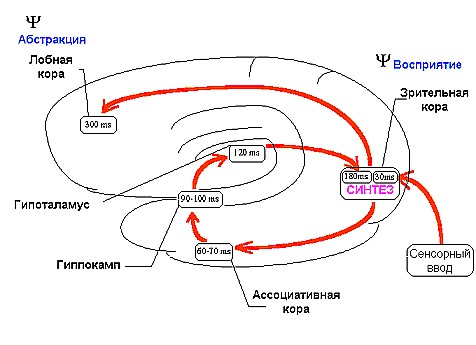
\includegraphics[width=0.7\linewidth]{ivanitsky_cyrcle}
		\caption{<<Круг ощущений>> по Иваницкому \cite{Aleksandrov2007}.}
		\label{fig:ivan_cyrcle}
	\end{figure}
	
	Говоря о современных представлениях о строении коры головного мозга, следует отметить, что оно практически однородно во всём своём объёме, о чём свидетельствует наличие макро- и миниколонок неокортекса \cite{Mountcastle1998,Rockland2010}. При этом связи между достаточно малыми зонами коры (так называемый коннектом \cite{Zador2012}) указывают на иерархичность её строения и на присутствие как восходящих, так и обратных, нисходящих связей. Отсюда следует, что основные компоненты элемента индивидуального знания должны обладать иерархическим однородным строением с восходящими потоками информации и нисходящей обратной связью. Известно также, что образная компонента должна реализоваться такой функцией распознавания, которая кроме категоризации процессов и статических объектов использует обратную связь для предсказания сигнала в следующий момент времени. Эти соображения будут использоваться для построения алгоритма формирования образной компоненты знака.
	
	\section{Модельный (или семантический) уровень}\label{sect:seman}
	Начнём с построения образа знака. Для этого будем использовать автоматы вида  $R=<A,Q,B,\varphi, \eta>$, где $A$ "--- множество входных сигналов, $B$ "--- множество выходных сигналов, $Q$ "--- множество состояний, $\varphi$ "--- функция переходов, $\eta$ "--- функция выходов. Такие автоматы, функционирующие по специальному нейрофизиологически правдоподобному алгоритму, будем называть распознающими или $R$-автоматами. 
	
	Пусть $\mathcal F$ "--- множество признаков. Входные и выходные сигналы будем задавать с помощью  векторов действительных чисел. Каждый элемент такого вектора является весом некоторого признака из $\mathcal F$. Для каждого распознающего автомата выделим два подмножества $F\subseteq\mathcal F$ и $F*\subseteq\mathcal F$, которые будем называть входными и выходными признаками соответственно. В общем виде работа автомата заключается в распознавании выходных признаков из множества $F$ по входному сигналу с помощью функций распознавания. Каждый из признаков $f_k\in F*$ распознаётся своей функцией распознавания $\hat f_k: X\rightarrow \mathbb R$.
	
	Работа функции распознавания $\hat f_k$ заключается в сопоставлении каждому признаку $f_k$ из множества $F^*$ действительного числа $x_k^*$, вычисляемого по вектору $\bar x$ входного сигнала. Значение $x_k^*$ определяет оценку успешности построения признака $f_k$ из составляющих его входных признаков, оценки которых во входном сигнале заданы вектором $\bar x$. В этом случае будем говорить, что распознающий автомат $R$ распознает признак $f_k$: $f_k\dashv R$.
	
	В соответствии с результатами нейрофизиологических исследований, приведёнными выше, будем считать, что множество  $\mathcal R$ распознающих автоматов образует иерархию "--- связный ориентированный ярусный граф. Некоторые части взвешенных векторов оценок выходных признаков распознающих автоматов $R_{i_1}^j,R_{i_2}^j,\dots,R_{i_q}^j$ путём конкатенации составляют вектор входных признаков для  автомата $R_k^{j+1}$ следующего уровня иерархии. Такой $R$-автомат $R_k^{j+1}$ будем называть родительским по отношению к автоматам $R_{i_1}^j,R_{i_2}^j,\dots,R_{i_q}^j$. Нижний индекс распознающего автомата нумерует автоматы из $\mathcal R$, а верхний обозначает номер яруса, которому принадлежит автомат.
		
	Рассмотрим более детально множества входных сигналов $A$, выходных сигналов $B$ и множества состояний $Q$.
	
	Входом $R$-автомата $R_i^j$ является множество пар векторов $(\bar x,\hat x^{j+1})$, где первый вектор пары является вектором размерности $q$ весов входных признаков, а второй "--- управляющим вектором размерности $l$ со следующего уровня иерархии, который принимает ненулевое значение только в фиксированные для данного автомата $R_i^j$ моменты времени $0,h,2h,\dots$. Таким образом, множество входных сигналов $A$ является декартовым произведением множеств векторов входных признаков $X$ и управляющих векторов со следующего уровня иерархии $\hat X^{j+1}$: $A=X\times \hat X^{j+1}$. 
	
	Выходом $R$-автомата также является множество пар $(\bar x^*,\hat x^j)$, где $\bar x^*$ "--- это вектор весов выходных признаков размерности $l$, а $\hat x^j$ "--- управляющий вектор размерности $q$ для предшествующего уровня иерархии, который наряду с выходами других автоматов уровня $j$ является входным управляющим вектором для некоторых автоматов уровня $j-1$. Таким образом, выходное множество $B$ также является декартовым произведением множеств взвешенных векторов выходных признаков $X^*$ и управляющих векторов для предшествующего уровня иерархии $\hat X^j$: $B=X^*\times \hat X^j$.
	
	Будем считать множество состояний конечным, в связи с чем каждой функции распознавания $\hat f_k$ из множества $\hat F$ поставим в соответствие набор матриц предсказания $Z_k=\{Z_1^k,…,Z_m^k\}$ размерности $q\times h$, где $h$ "--- глубина памяти распознающего автомата, играющая также роль характерного времени. Столбец $\bar{z}_u^r=(z_{u1}^k,…,z_{uq}^k)$ матрицы $Z_r^k$ есть вектор предсказания присутствия во входном векторе признаков из множества $F$ в моменты времени $\tau+u$, где $\tau = 0,h,2h,\dots$. При этом $z_{uv}^k\in\{0,1\}$, т.~е. вектор $\bar{z}_u^r$ является булевым вектором. Сама матрица $Z_r^k$ задаёт, таким образом, последовательность событий, наличие которых свидетельствует о~присутствии распознаваемого функцией $\hat f_k$ признака. Иными словами, множество всех матриц предсказания $\mathcal Z$ распознающего автомата хранит в себе информацию о выходных признаках. Множество состояний автомата тогда является булеаном множества матриц предсказания: $Q=2^{\mathcal Z}$.
	
	Алгоритм $\mathcal A_{th}$ вычисления функции переходов $\varphi:X\times\hat X^{j+1}\to 2^{\mathcal Z}$ и выходной функции $\eta:2^{\mathcal Z}\to X^*\times\hat X$ по начальному моменту времени $\tau$, управляющему воздействию $\hat x^{j+1}(\tau)$ и входному воздействию $\omega:T\to X$ представлен ниже. В алгоритме используется стандартная функция $W$ нормировки значений весов:
	\begin{equation}
	W(\bar x)=\left(\frac{x_1}{\max\limits_i x_i},\dots,\frac{x_n}{\max\limits_i x_i}\right),
	\end{equation} 
	где $\bar x=(x_1,\dots,x_n)$ "--- вектор с ненормированными компонентами.

	\renewcommand{\baselinestretch}{1}
	\begin{algorithm}[h]
		\caption{Алгоритм $\mathfrak{A}_{th}$ вычисления автоматной функции распознающего автомата $R_i^j$}\label{alg:automato}
		\begin{algorithmic}[1]
					\Require $\tau_s, \hat{x}_i^{j+1}(\tau_s), \omega_i^j$.
		\Ensure $\varphi_{i\Delta t}^j, \vec\eta_{i\Delta t}^j$.

		\State $\hat{F}^*=\varnothing,Z^*=\varnothing,t=0$; \Comment{активные функции распознавнаия и матрицы предсказания}
		\State $c_1\in(0,1), c_2\in(0,1)$; \Comment{пороговые константы}

		\Statex \Comment{определение начального состояния}
				
		\ForAll{компонент $\hat{x}_{ik}^{j+1}$ вектора $\hat{x}_i^{j+1}(\tau_s)=(\hat{x}_{i1}^{j+1},\hat{x}_{i2}^{j+1},\dots,\hat{x}_{il}^{j+1})$} \label{alst:init_start}
			\If{$\hat{x}_{ik}^{j+1}{\ge}c_1$} \label{alst:select_f}
				\State $\hat{F}^*:=\hat{F}^*\cup\{\hat{f}_k\}$;
			\EndIf
		\EndFor
		
		\State $\bar x_i^j:=\omega_i^j(\tau_s)$;
		
		\ForAll{функций распознавания $\hat{f}_k\in\hat{F}^*$}
			\ForAll{$Z_r^k\in Z_k$, соответствующих функции распознавания $\hat{f}_k$,}
				\If{$\frac{\|\bar{z}_1^r-\bar{x}_i^j\|}{\|\bar{z}_1^r\|+\|\bar{x}_i^j\|}<c_2$} \label{alst:select_z}
					\State $Z^*:=Z^*\cup\{Z_r^k\}$;
				\EndIf
			\EndFor
		\EndFor
		
		\State $\varphi_i^j(\bar x_i^j,\hat{x}_i^{j+1}(\tau_s)) := Z^*$; \Comment{значение функции переходов в начальный момент времени}\label{alst:init_state}
		\State $\bar N:=(|\{Z_r^1|Z_r^1\in Z^*\}|,\dots,|\{Z_r^{l_i^j}|Z_r^{l_i^j}\in Z^*\}|)$; \label{alst:init_calc_out2}
		\State $\eta(Z^*)=\bar{x}_i^{*j}:=W(\bar N)$; \Comment{значение функции выходов в начальный момент времени} \label{alst:init_calc_out3}
		\State $\hat x_i^j=W(\sum_{\hat f_k\in\hat F^*}\hat x_{ik}^{j+1}\sum_{Z_r^k\in Z^*}\bar z_2^r)$;\label{alst:init_control}
		\label{alst:init_end}
				\Statex \Comment{основной цикл}
	
	\State $t=1$;
	\While{$t\leqslant{h_i^j}-1$} \label{alst:cycle_start}
		\State $\bar{x}_i^j:=\omega(\tau_s+t)$;
	
		\ForAll{матриц предсказания $Z_r^k$ из множества $Z^*$}
			\If{$\frac{\|\bar{z}_{t+1}^r-\bar{x}_i^j\|}{\|\bar{z}_{t+1}^r\|+\|\bar{x}_i^j\|}\geqslant{c_2}$} \label{alst:update_z}
				\State $Z^*:=Z^*\setminus\{Z_r^k\}$;
			\EndIf
		\EndFor
	
		\State $\varphi_i^j(\bar x_i^j,\hat{x}_i^{j+1}(\tau_s)) := Z^*$; \Comment{значение функции переходов в момент времени $t$}
		\State $\bar N=(|\{Z_r^1|Z_r^1\in Z^*\}|,\dots,|\{Z_r^{l_i^j}|Z_r^{l_i^j}\in Z^*\}|)$; \label{alst:calc_out1}
		\State $\eta(Z^*)=\bar{x}_i^{*j}:=W(\bar N)$;\Comment{значение функции выходов в момент времени $t$} \label{alst:calc_out3}
	
		\State $t=t+1$;
		\If{$t\leqslant{h}_i^j-2$}
			\State $\hat{x}_i^j:=W(\sum_{\hat f_k\in\hat F^*}\hat x_{ik}^{j+1}\sum_{Z_r^k\in Z^*}\bar z_t^r)$; \label{alst:calc_state1}
		\EndIf
	\EndWhile \label{alst:cycle_end}
		\end{algorithmic}
	\end{algorithm}
	\renewcommand{\baselinestretch}{\stretchsize}

	Вследствие особенностей алгоритма $\mathcal A_{th}$ и  того, что множества входных и выходных сигналов являются векторными пространствами, распознающий автомат $R$ является бесконечным автоматом Мили с переменной структурой и конечной памятью (рис. \ref{fig:rb_io}): 
	\begin{equation}
	R_i^j=<X\times\hat X^{j+1}, 2^{\mathcal Z}, X^*\times\hat X^j,\varphi_i^j,\eta>.
	\end{equation}

	\begin{figure}[h]
		\centering
		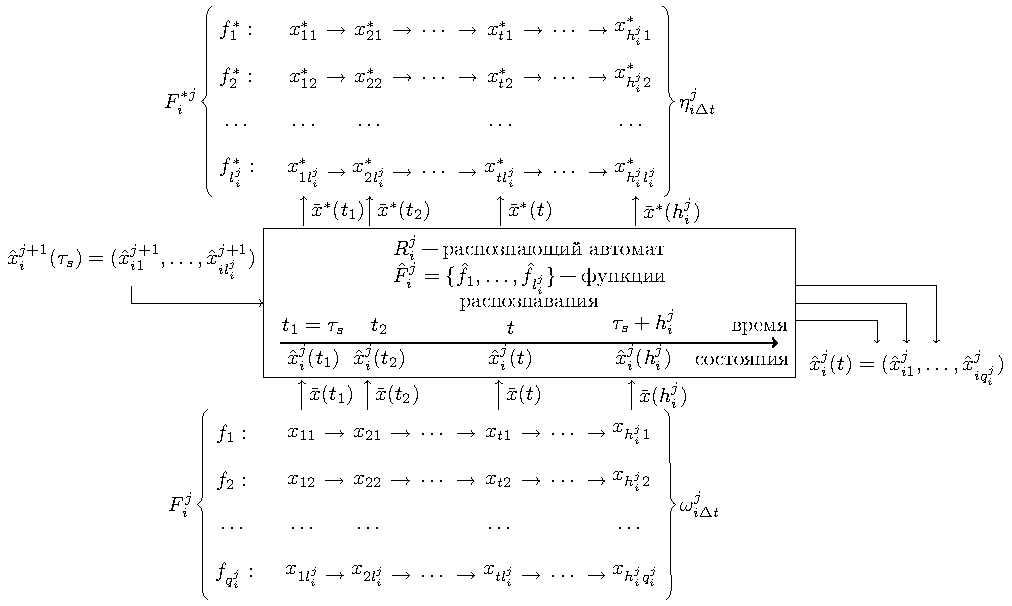
\includegraphics[width=1.0\linewidth]{rb_io}
		\caption{Вход и выход распознающего автомата $R_i^j$.}
		\label{fig:rb_io}
	\end{figure}

	\subsection{Процедурные и объектные признаки}
	Далее будет дано определение значения знака на семантическом уровне с помощью множества правил, каждое из которых соответствует некоторому действию. Правило будем представлять в виде пары <<условие "--- эффект действия>> так, как это понимается в искусственном интеллекте \cite{Nilson1985}. Для связи правил и распознающих автоматов необходимо ввести ряд вспомогательных определений. 

	В~начале следует отметить, что каждый элемент векторов"--~столбцов соотносится с~признаком из~входного множества признаков распознающего автомата, что означает задание индекса для каждого входного признака. Индекс признака $f_k\in F_i^j$ равен  $q$, если ему соответствует $q$-ый элемент векторов"--~столбцов матриц предсказания распознающего автомата $R_i^j$. 
	
	Введём семейство бинарных отношений $\{\sqsubset,\sqsubset^1,\sqsubset^2,\dots\}$, определённых на декартовом произведении $\mathcal F\times \mathcal F$. Будем считать, что <<признак $f_1$ поглощается признаком $f_2$>> $f_1\sqsubset f_2$ в том случае, если $f_1\dashv R_i^j, f_2\dashv R_q^{j+1}$, $R_q^{j+1}$ "--- родительский автомат по отношению к $R_i^j$ и в множестве матриц предсказания $\mathcal Z_2$ признака $f_2$ существует хотя бы одна матрица $Z_r^2$, содержащая некоторый столбец $\bar z_u^r$ с элементом $z_{uv}^r=1$, где $f_q^{j+1}(v)=f_1$ (см. рис. \ref{fig:auto_measur}).
		
	\begin{figure}[h]
		\centering
		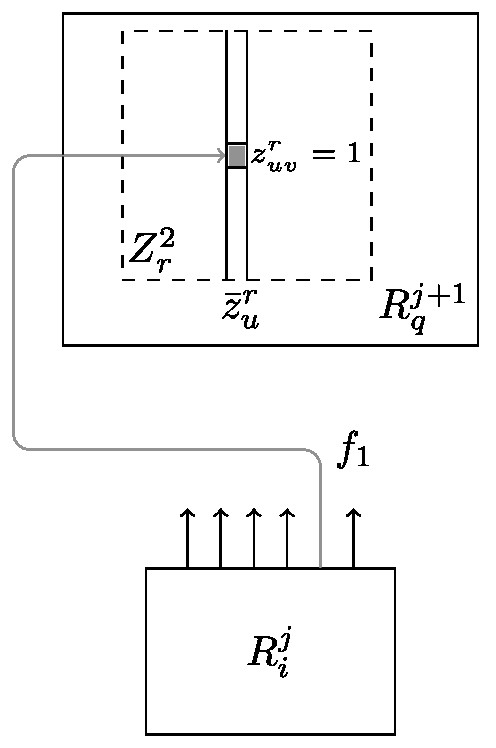
\includegraphics[width=0.3\linewidth]{automata/meas}
		\caption{Схема определения отношения поглощения признаков $f_1$ и $f_2$: $f_1\sqsubset f_2$.}
		\label{fig:auto_measur}
	\end{figure}
			
	Пара признаков $(f_1,f_2)$ принадлежат отношению $\sqsubset^t$, т.~е. $f_1\sqsubset^t f_2$, где $t\in\{1,2,\dots\}$, в~том случае, если $f_1\dashv R_i^j, f_2\dashv R_q^{j+1}$, $R_q^{j+1}$ "--- родительский автомат по отношению к $R_i^j$ и в множестве матриц предсказания $Z_2$ признака $f_2$ существует хотя бы одна матрица $Z_r^2$, содержащая $t$–ый столбец $\bar z_t^r$ с~элементом $z_{tv}^r=1$, где $f_q^{j+1}(v)=f_1$.	
	
	Введём операцию $\Lambda$, которая по множеству матриц распознавания $\mathcal Z_k$ признака $f_k$ определяет два набора индексов столбцов матриц из $Z_k$. Первый набор $I_c=\{i_1^c,i_2^c,\dots\}$, $\forall k\ 0\leqslant i_k^c < h$, составляют индексы \textit{столбцов условий}, в которых ненулевые элементы определяют условия проявления признака $f_k$. Второй набор $I_e=\{i_1^e,i_2^e,\dots\}$, $\forall k\ 0\leqslant i_k^e < h$, состоит из индексов  \textit{столбцов эффектов}, в которых ненулевые элементы определяют эффекты проявления признака $f_k$. Примером реализации процедуры $\Lambda$ может служить алгоритм Норриса по поиску максимального прямоугольного подмножества в бинарном отношении \cite{Norris1977}.
	
	Признаки, для матриц предсказания которых процедура $\Lambda$ выдаёт не пустые множества индексов $I_c$ и $I_e$, будем называть процедурными признаками, остальные "--- объектными признаками. Это означает, что всё множество признаков делится на два подмножества: $\mathcal F=\mathcal F^{proc}\cup\mathcal F^{obj}$ и $\mathcal F^{proc}\cap\mathcal F^{obj}=\varnothing$.	

	Для любого процедурного признака выполняются следующие естественные условия:
	\begin{itemize}
		\item условие всегда предшествует эффекту,
		\item условие всегда влечёт за собой эффект и
		\item все условия всегда отделены от своих эффектов.
	\end{itemize}
		
	Иными словами, если $f_1$ "--- процедурный признак, то если столбец $\bar z_u^r$ матрицы предсказания $Z_r^1$ является столбцом условий, т.~е. $u\in{I_c}$, этот столбец не может одновременно являться столбцом эффектов, т.~е. $u\not\in I_e$, и существует такое $t>0$, что столбец $\bar z_{u+t}^r$ является столбцом эффектов, т.~е. $u+t\in I_e$.
		
	Пополним семейство отношений $\{\sqsubset,\sqsubset^1,\sqsubset^2,\dots\}$ двумя отношениями: $\sqsubset^c$ и $\sqsubset^e$, принадлежность к~которым пары признаков $(f_1,f_2)$ свидетельствует о~том, что признак $f_1$ присутствует соответственно в~столбце условий и эффектов как минимум в~одной матрице предсказания процедурного признака $f_2$.
		
	\subsection{Определение компонент знака}
	Пусть $S$ "--- множество знаков. Будем считать, что будущему знаку $s\in S$ \textit{соответствует} некоторый признак $f(s)\in\mathcal F$, обладающий перцептом $\tilde p$, функциональным значением $\tilde m$ и биологическим смыслом $\tilde a$, которые после завершения процесса формирования знака $s$ становятся, соответственно, образом $p$, значением $m$ и личностным смыслом $a$.
	
	\begin{Def}
		Если $f_1$ "--- признак, соответствующий знаку $s_1$, то подмножество $\tilde p(f_1)\subseteq\mathcal F$ таких признаков, что $\forall f_i\in\tilde p(f_1) f_i\sqsubset f_1$, будем называть перцептом признака $f_1$.
	\end{Def}
	
	На множестве всех перцептов $\tilde P$ введём метрику $\rho_p(\tilde p(f_1),\tilde p(f_2))$, вычисляемую по~следующему правилу:
	\begin{itemize}
		\item если $f_1$ и $f_2$ распознаются разными $R$-автоматами, т.~е. $f_1\dashv R_i^j, f_2\dashv R_q^k$, то $\rho_p(\tilde p(f_1),\tilde p(f_2))=\infty$,
		\item если $f_1$ и $f_2$ распознаются одним и тем~же $R$-автоматом $R_i^j$ со~множеством входных признаков $F_i^j$ мощности $q$ и характерным временем $h$, то
		\begin{equation}
			\rho_p(\tilde p(f_1),\tilde p(f_2))=\min\limits_{\substack{Z_r^1\in Z_1\\Z_s^2\in Z_2}}\frac{1}{q\cdot h}\sum\limits_{u=1}^h\|\bar z_u^r-\bar z_u^s\|.
		\end{equation} 
	\end{itemize}
	
	\begin{Def}
		Если $f_1$ "--- признак, соответствующий знаку $s_1$, $f_2$ "--- процедурный признак, $f_1\sqsubset^c f_2$, то будем называть $f_2$ элементом функционального значения признака $f_1$. Множество всех элементов функционального значения признака $f_1$ будем обозначать $\tilde m(f_1)$.
	\end{Def}
	
	На множестве всех функциональных значений $\tilde M$ введём метрику $\rho_m(\tilde m(f_1),\tilde m(f_2))$, вычисляемую по следующему правилу:
	\begin{equation}\label{eq:m_metr}
		\rho_m(\tilde m_1(f_1),\tilde m_2(f_2 ))=\min\limits_{\substack{f_i\in\tilde m(f_1 )\\f_j\in\tilde m(f_2 )}}\rho_p(\tilde p(f_i ),\tilde p(f_j )).
	\end{equation}
		
	Самосознание субъекта деятельности включает в себя выделенный знак $s_I$, являющийся представлением субъекта о самом себе. То множество признаков которое составляет образ знака $s_I$ будем называть личностными признаками и выделять в специальное подмножество $F_I\subset\mathcal F$.
	
	\begin{Def}\label{def:meaning}
		Если $f_1$ "--- признак, соответствующий знаку $s_1$, $f_2$ "--- процедурный признак, $f_1\sqsubset^c f_2$, такой, что $F_C(f_1)\cap F_I\not = \varnothing$, то будем называть $f_2$ элементом биологического смысла признака $f_1$. Множество всех элементов биологического смысла признака $f_1$ будем обозначать $\tilde a(f_1)$.
	\end{Def}
	
	\subsection{Семантический уровень обобщения} На основе описанной модели компонент знака становится возможным описать процедуры обобщения (см. первую часть работы) на модельном, семантическом уровне. Для этого будем считать, что матрицы предсказания распознающих автоматов были сформированы в процессе обучения (например, с использованием алгоритма HTM \cite{Hawkins2009} или THSOM \cite{Koutn2008}). При рассмотрении множества матриц предсказания $\mathcal Z$ некоторого распознающего автомата возникают следующие три основных случая:
	\begin{itemize}
		\item \textit{Внутреннее обобщение}. Будем называть схожими, такие матрицы из подмножества $Z'_k=\{Z_1^k,Z_2^k\dots,Z_m^k\}$ множества матриц предсказания $Z_k$ некоторого признака $f_k$, для которых при $\forall i,j,l$ таких, что $Z_i,Z_j\in Z'_k,l\in\{0,\dots,h\}$ выполняется $card(z_l^i\wedge z_l^j)<c_3$, где $c_3$ "--- некоторая константа. Обобщение в этом случае заключается в замене подмножества схожих матриц $Z'_k$ одной обобщённой $Z^*=(\bigwedge\limits_{Z_q\in Z'_k}\bar z_1^q,\bigwedge\limits_{Z_q\in Z'_k}\bar z_2^q,\dots,\bigwedge\limits_{Z_q\in Z'_k}\bar z_h^q)$. Таким образом, осуществляется кластеризация множества матриц предсказания признака $f_k$, контролируемая одним параметром близости $c_3$.
		\item \textit{Конкретизация}. В~тех случаях, когда получаемые с использованием описанной выше меры близости кластеры матриц предсказания признака $f_k$ расходятся достаточно сильно, образуются новые конкретизированные признаки для каждого кластера и соответственно расширяется множество выходных признаков $F^*$ распознающего автомата.
		\item \textit{Внешнее обобщение}. В~том случае когда во~всех матрицах предсказания $R$-автоматов, являющихся родительскими по отношению к распознающему автомату $R$, $i$-ые и $j$-ые компоненты всех столбцов матриц принимают одинаковые значения, выходные признаки $f_i,f_j\in F^*$, соответствующие этим компонентам, обобщаются в один признак с объединённым множеством матриц предсказания. При этом возможно и дальнейшее внутреннее обобщение.
	\end{itemize}
	
	Отдельно необходимо рассмотреть случай \textit{абстрагирования}, когда несколько выходных признаков одного или нескольких распознающих автоматов в результате работы процедуры обобщения на синтаксическом уровне (см. первую часть работы) формируют новый признак $f^*$ в некотором $R$-автомате $R^*$, лежащем на следующем уровне иерархии. В этом случае матрица предсказания будет состоять из единственного столбца с ненулевыми элементами, которые соответствуют признакам, составляющим данную категорию.
	
	И, наконец, ещё один случай обобщения на семантическом уровне заключается в образовании ролевой структуры процедурных признаков. Рассмотрим случай, когда столбцы условий или эффектов некоторых матриц предсказания процедурного признака $f_p$ различаются только в двух компонентах, т.~.е. $i$-ая компонента в некоторых столбцах равна $1$, а в других "--- $0$, а $j$-ая компонента наоборот "--- в первых равна $0$, а во вторых "--- $1$. Если соответствующие этим компонентам признаки в результате абстрагирования попали в некоторую общую категорию $f_{cat}$, то к множеству матриц предсказания признака $f_p$ добавляется матрица с новой компонентой, соответствующей признаку $f_{cat}$ и обнулёнными компонентами $i$ и $j$. Данная процедура легко распространяется на случай, когда количество элементов категории $f_{cat}$ в матрицах предсказания признака $f_p$ больше двух. Таким образом, для процедурного признака $f_p$ появляется обобщённая, ролевая матрица предсказания.

	\section{Формирование значения знака} \label{sect:link}
	В начале подробнее рассмотрим строение матрицы предсказания $Z_r^p$ некоторого процедурного признака. Легко показать, что эту матрицу можно представить в следующем виде:
	\begin{equation}
	Z_r^p=(\bar z_1^{r,c},\dots,\bar z_{j_1}^{r,c},\bar z_{j_{1+1}}^{r,e},\dots,\bar z_{i_1}^{r,e},\dots,\dots,\bar z_{i_{k-1}+1}^{r,c},\dots,\bar z_{j_k}^{r,c},\bar z_{j_k+1}^{r,e},\dots,\bar z_{i_k}^{r,e}),
	\end{equation}
	где $\bar z_j^{r,c}$ "--- столбцы причин, $\bar z_i^{r,e}$ "--- столбцы следствий. 
	
	Величину $k$ будем называть \textit{сложностью} процедурного признака. В~дальнейшем будем рассматривать простые матрицы предсказаний $k$-сложного процедурного признака:
	\begin{equation}
	Z_r^p=(\bar z_1^{r,c},\bar z_2^{r,e},\dots,\dots,\bar z_{2\cdot k-1}^{r,c},\bar z_{2\cdot k}^{r,e}).
	\end{equation}
	Краткая форма $k$-сложного процедурного признака $f_p$ имеет матрицу предсказания, в которой оставлены только первый столбец условий и последний столбец эффектов.
	
	Любой процедурный признак $f_p$ со сложностью $k=1$ (элементарный), распознаваемый автоматом $R_i^j$, можно представить в виде правила $r_p=(F_C(f_p),F_A(f_p),F_D(f_p))$, в котором:
	\begin{itemize}
		\item $F_C (f_p )\subseteq F_i^j$ "--- множество признаков "--- условий правила: $\forall f\in F_C(f_p)$ $f\sqsubset^c f_p$;
		\item $F_A(f_p)\subseteq F_i^j$ "--- множество добавляемых правилом признаков: $\forall f\in F_A(f_p)$ $f\sqsubset^e f_p,f\not\sqsubset^c f_p$;
		\item $F_D(f_p)\subseteq F_i^j$ "--- множество удаляемых правилом признаков: $\forall f\in F_D(f_p)$ $f\not\sqsubset^e f_p,f\sqsubset^c f_p$.
	\end{itemize}
	
	Очевидно, выполняются следующие соотношения: $F_A(f_p)\cap F_D(f_p)=\varnothing, F_A(f_p)\cap F_C(f_p)=\varnothing, F_D(f_p)\subseteq F_C(f_p)$.

	\begin{Def}\label{def:feas}
		Процедурный признак $f_p^1\dashv R_i^j$ c матрицей предсказания $Z=(\bar z_1^c,\bar z_2^e)$ выполняется на векторе $\bar z$ длины $q$, где $q$ "--- длина входного вектора $R$-автомата $R_i^j$, если $\bar z\cdot \bar z_1^c=\bar z_1^c$.
	\end{Def}
	
	Здесь под операцией <<$\cdot$>> подразумевается покомпонентное умножение битовых векторов. Если в качестве вектора $\bar z$ в определении (\ref{def:feas}) взять столбец условий некоторого признака $f_p^2$, то будем говорить, что процедурный признак $f_p^1$ выполним в~условиях процедурного признака $f_p^2$, если 
	\begin{itemize}
		\item оба признака распознаются одним и тем~же распознающим автоматом $R_i^j$ и признак  $f_p^1$ выполняется на~столбце условий матрицы предсказания признака $f_p^2$,
		\item $f_p^1\dashv R_i^{j_1}, f_p^2\dashv R_k^{j_2}$, $i\not=k$, $F_C(f_p^1 )\subseteq F_C(f_p^2)$ и признак  $f_p^1$ выполняется на~столбце условий матрицы предсказания признака $f_p^2$. 
	\end{itemize}
	
	\begin{Def}
		Будем говорить, что два процедурных признака $f_p^1$ и $f_p^2$ конфликтуют, если выполнено как минимум одно из~следующих условий:
		\begin{itemize}
			\item $F_D(f_p^1)\cap F_A(f_p^2)\not=\varnothing$,
			\item $F_D(f_p^2)\cap F_A(f_p^1)\not=\varnothing$,
			\item $F_D(f_p^1)\cap F_C(f_p^2)\not=\varnothing$,
			\item $F_D(f_p^2)\cap F_C(f_p^1)\not=\varnothing$.
		\end{itemize}
	\end{Def}
	
	\begin{Def}
		Результатом операции приведения вектор"--~столбца $\bar z$ матрицы распознавания $R$-автомата $R_{i_1}^{j_1}$ к $R$-автомату $R_{i_2}^{j_2}$ будем называть такой вектор $\bar z'$ длины $q_{i_2}^{j_2}$, $k$-ый элемент которого $z'_k=1$, если признак $f\in F_{i_1}^{j_1}$ с индексом $k$ равен признаку $f'\in F_{i_2}^{j_2}$ с тем же индексом и $z_k=1$, иначе $z'_k=0$, и обозначать его $(\bar z\rightarrow R_{i_2}^{j_2})=\bar z'$.
	\end{Def}
	
	\begin{Def}
		Результатом операции приведения вектор"--~столбца $\bar z$ матрицы распознавания $R$-автомата $R_{i_1}^{j_1}$ к $R$-автомату $R_{i_2}^{j_2}$ по столбцу $\bar z'$ матрицы распознавания из множества  $\mathcal Z_{i_2}^{j_2}$ будем называть такой вектор $\bar z''$ длины $q_{i_2}^{j_2}$, элемент которого $z''_k=1$, если признак $f\in F_{i_1}^{j_1}$ с индексом $k$ равен признаку $f'\in F_{i_2}^{j_2}$ с тем же индексом, $z'_k=1$ и $z_k=1$, иначе $z''_k=0$, и обозначать $(\bar z\xrightarrow{\bar z'} R_{i_2}^{j_2})=\bar z''$.
	\end{Def}

	
	\subsection{Алгоритм связывания образа и значения знака}
	Будем считать, что у субъекта имеется опыт наблюдения, который выражается в виде функции $\Psi_p^m$. $\Psi_p^m(\tilde p)=\tilde m$, в том случае, если $\tilde p\in\tilde P$ является перцептом некоторого признака $f$, а $\tilde m\in\tilde M$ "--- функциональным значением того же признака $f$.
	
	Ниже представлен алгоритм доопределения функции $\Psi_p^m$, который и отражает собой суть процесса во время образования знака согласно алгоритму из первой части работы. Доопределение проводится на~новую пару $(\tilde p,\tilde m)$, где функциональное значение $\tilde m$ строится в сравнении с эталоном $\tilde m^0$, а перцепт $\tilde p$ формируется на основе области определения $\hat F$ функции $\Psi_p^m$. Доопределение функции $\Psi_p^m$ означает формирование нового признака $f^*$, т.~е. его первой матрицы предсказания $Z^*$ в~рамках распознающего автомата $R^*$.

	\renewcommand{\baselinestretch}{1}				
	\begin{algorithm}[h]
		\caption{Алгоритм $\mathfrak{A}_{pm}$ (часть I)}
		\label{alg:cycle_pm_start}
		\begin{algorithmic}[1]
				\Require $\tilde m^0=\{f_p^0\}, \Psi_p^m, \hat F=dom\ \Psi_p^m\subseteq \mathcal F$;
	\algrule
	\State $Z_p^0 := \{\bar z_1^{c0},\bar z_2^{e0}\}$ "--- матрица предсказания признака $f_p^0$;
	\State $\tilde p^{(0)} := \varnothing$, $\tilde m^{(0)} := \varnothing$;
	\State $R_0\not\in\mathcal R$ "--- фиктивный распознающий блок, для которого $F_0^*=\{f_p^0\}$;
	\State $Z^{(0)} := \varnothing$, $Z_p^{(0)} := \{\bar 0, \bar 0\}$;
	\State $q^{(0)} := 0$, $t := 0$;
	
	\While{$Z_p^{(t)}\not=Z_p$ или $t<|\hat F|$}
		\State $f\in\hat F$ "--- первый не рассмотренный ранее признак; 
		\State $Z=\{\bar z_1,\bar z_2,\dots,\bar z_q\}$ "--- его матрица предсказания;
		\If{$\exists \tilde m=\{f_p\}\in \tilde M$ такое, что $(\tilde p(f),\tilde m)\in\Psi_p^m$, $f_p$ выполним в условиях признака $f_p^0$ и $\nexists f'$ такого, что $f'\in\tilde p^{(t)}$,$\tilde m'=\{f'_p\}\in\tilde M$, $(\tilde p(f'),\tilde m')\in\Psi_p^m$, $f'_p$ конфликтует с $f_p$}\label{alst:find_m}
			\State $\tilde p^{(t+1)}=\tilde p^{(t)}\cup\{f\}$;
			\State $Z_p=\{\bar z_1^{c},\bar z_2^{e}\}$ "--- матрица предсказания признака $f_p$;
	
			\If{$\exists R_i^j$ такой, что $\tilde p^{(t+1)}\subseteq F_i^j$}
				\State $R_i^{j(t+1)}:=R_i^j$;
			\Else
				\State $R_i^{j(t+1)}:=\argmax\limits_{\mathcal R} (F_i^j\cap\tilde p^{(t+1)})$;
				\State $F_i^{j(t+1)}:=F_i^{j(t)}\cup\tilde p^{(t+1)}$;
			\EndIf

			\algstore{algst:store2}
		\end{algorithmic}			
	\end{algorithm}
	\renewcommand{\baselinestretch}{\stretchsize}

	\renewcommand{\baselinestretch}{1}				
	\begin{algorithm}[h]
		\caption{Алгоритм $\mathfrak{A}_{pm}$ (часть II)}
		\label{alg:cycle_pm_end}
		\begin{algorithmic}[1]
			\algrestore{algst:store2}
						\State $q^{(t+1)}=\max\{q^{(t)},q\}$;
			\State $Z^{(t+1)}:=\{\bar z_1^{(t+1)},\bar z_2^{(t+1)},\dots \bar z_{q^{(t+1)}}^{(t+1)}\}$, где $\bar z_i^{(t+1)}=\bar z_i^{(t)}\vee \bar z_i$, если $i\leqslant q$ и $i\leqslant q^{(t)}$, $\bar z_i^{(t+1)}=\bar z_i^{(t)}$, если $i>q$ и $\bar z_i^{(t+1)}=\bar z_i$, если $i > q^{(t)}$;
			
			\State $Z_p^{(t+1)}:=\{\bar z_1^{c(t+1)},\bar z_2^{e(t+1)}\}$, где $\bar z_1^{c(t+1)}=\bar z_1^{c(t)}\vee (\bar z_1^c\rightarrow R_0)$, $\bar z_2^{e(t+1)}=\bar z_2^{e(t)}\vee (\bar z_2^e\xrightarrow{\bar z_2^{e0}} R_0)$;
			
			\State $f_p^{(t+1)}$ "--- признак с матрицей предсказания $Z_p^{(t+1)}$;
			
			\State $\tilde m^{(t+1)}=\{f_p^{(t+1)}\}$;
		\EndIf
	
		\State $t=t+1$;
	\EndWhile

	\State $R^*=R_i^{j(t)}$;
	\State $Z^*=Z^{(t)}$;
	\State $\mathcal Z^{*}=\mathcal Z_i^{j(t)}\cup\{Z^*\}$;	
	
	\Return $\Psi_p^m$, доопределённую на паре $(\tilde p, \tilde m)$, где $\tilde p=\tilde p^{(t)}$, $\tilde m=\tilde m^{(t)}$.
		\end{algorithmic}		
	\end{algorithm}
	\renewcommand{\baselinestretch}{\stretchsize}
		
	\begin{Theorem}[о корректности алгоритма $\mathfrak A_{pm}$]
		Алгоритм $\mathfrak A_{pm}$ корректен, т.~е. элементы последовательности функциональных значений $\langle\tilde m^{(0)},\tilde m^{(1)},\dots,\tilde m^{(t)}\rangle$, которая строится с помощью алгоритма $\mathfrak A_{pm}$ для функционального значения $\tilde m^0$, приближаются к $\tilde m^0$ в смысле метрики (\ref{eq:m_metr}).
	\end{Theorem}
	
	\begin{Proof}
		Рассмотрим два элемента последовательности $\tilde m^{(t)}=\{f_p^{(t)}\}$ и $\tilde m^{(t+1)}=\{f_p^{(t+1)}\}$. Соответствующие матрицы предсказания будут иметь следующий вид:
		\begin{equation}
		Z_p^{(t)}=\{\bar z_1^{c(t)},\bar z_2^{e(t)}\},\ Z_p^{(t+1)}=\{\bar z_1^{c(t+1)},\bar z_2^{e(t+1)}\}.
		\end{equation}
		Если на шаге \ref{alst:find_m} алгоритма $\mathfrak A_{pm}$ на $(t+1)$-й итерации не был найден подходящий признак, то матрицы $Z_p^{(t)}$ и $Z_p^{(t+1)}$ равны. Рассмотрим случай, когда был найден подходящий признак $f'$ с функциональным значением $\tilde m'=\{f'_p\}$ с соответствующей матрицей предсказания $Z'=(\bar z'^c_1,\bar z'^e_2)$.
		
		В том случае, если на шаге \ref{alst:find_m} был найден признак $f'_p$ то матрицы $Z_p^{(t)}$ и $Z_p^{(t+1)}$ будут отличать в своих двух столбцах:
		\begin{equation}
		\bar z_1^{c(t+1)}=\bar z_1^{c(t)}\vee (\bar z'^c_1\rightarrow R_0),\ \bar z_2^{e(t+1)}=\bar z_2^{e(t)}\vee (\bar z'^e_2\xrightarrow{\bar z_2^{e0}} R_0).
		\end{equation}
		По определению расстояние между функциональными значениями $\tilde m^{(t)}$ и $\tilde m^0$ примет следующее значение:
		\begin{eqnarray}
		\rho_m(\tilde m^{(t)},\tilde m^0)=\min\limits_{\substack{f_i\in\tilde m^{(t)}\\f_j\in\tilde m^0}}\rho_p(\tilde p(f_i),\tilde p(f_j ))=\rho_p(\tilde p(f'_p),\tilde p(f_p))=\nonumber \\
		=\frac{1}{q\cdot h}\sum\limits_{\substack{\bar z_u^{1(t)}\in Z_p^{(t)}\\\bar z_u^2\in Z_p^0}}\|\bar z_u^{1(t)}-\bar z_u^2\|.
		\end{eqnarray}
		Аналогично для $\tilde m^{(t+1)}$:
		\begin{equation}
		\rho_m(\tilde m^{(t+1)},\tilde m^0)=\frac{1}{q\cdot h}\sum_{\substack{\bar z_u^{1(t+1)}\in Z_p^{(t+1)}\\\bar z_u^2\in Z_p^0}}\|\bar z_u^{1(t+1)}-\bar z_u^2\|.
		\end{equation}
		Рассмотрим разность 
		\begin{eqnarray}
		\rho_m(\tilde m^{(t)},\tilde m^0)-\rho_m(\tilde m^{(t+1)},\tilde m^0)=\frac{1}{q\cdot h}(\|\bar z_1^{c(t)}-\bar z_1^{c0}\|+\|\bar z_2^{e(t)}-\bar z_2^{e0}\|-\nonumber \\
		-\|\bar z_1^{c(t+1)}-\bar z_1^{c0}\|-\|\bar z_2^{e(t+1)}-\bar z_2^{e0}\|)=\frac{1}{q\cdot h}(\|\bar z_1^{c(t)}-\bar z_1^{c0}\|+\nonumber \\
		+\|\bar z_2^{e(t)}-\bar z_2^{e0}\|-\|\bar z_1^{c(t)}\vee (\bar z'^c_1\rightarrow R_0)-\bar z_1^{c0}\|-\nonumber \\
		-\|\bar z_2^{e(t)}\vee (\bar z'^e_2\xrightarrow{\bar z_2^{e0}} R_0)-\bar z_2^{e0}\|),
		\end{eqnarray}
		где $\bar z_1^{c0}$, $\bar z_2^{e0}$ "--- столбцы матрицы предсказания процедурного признака $f_p^0$, соответствующего функциональному значению $\tilde m^0$.
		
		Так как $f'_p$ выполним на первом столбце матрицы предсказания признака $f_p^0$, то после применении операции приведения $\bar z'^c_1\rightarrow R_0$ в результирующем векторе единицы появляются только на тех же местах что и в векторе $\bar z_1^{c0}$. Это означает, что в векторе $\bar z_1^{c(t)}\vee (\bar z'^c_1\rightarrow R_0)-\bar z_1^{c0}$ по сравнению с вектором $\bar z_1^{c(t)}$  единицы находятся только в тех же местах, что и в векторе $\bar z_1^{c0}$, а новых нулей не появляется. В следствие чего разность $\|\bar z_1^{c(t)}-\bar z_1^{c0}\|-\|\bar z_1^{c(t)}\vee (\bar z'^c_1\rightarrow R_0)-\bar z_1^{c0}\|$ всегда больше либо равна нулю.
		
		Так как для столбцов эффектов применяется операция приведения по столбцу, то единицы в результирующем векторе остаются только на тех местах, на которых одновременно находятся единицы в приводимом векторе и векторе, по которому осуществляется приведение. В связи с этим разность $\|\bar z_2^{e(t)}-\bar z_2^{e0}\|-\|\bar z_2^{e(t)}\vee (\bar z'^e_2\xrightarrow{\bar z_2^{e0}} R_0)-\bar z_2^{e0}\|$ также больше либо равна нулю.
		
		Так как обе разности в скобках выражения для $\rho_m(\tilde m^{(t)},\tilde m^0)-\rho_m(\tilde m^{(t+1)},\tilde m^0)$ больше либо равны нулю, то отсюда следует, что функциональное значение $\tilde m^{(t+1)}$ ближе или по крайней мере находится на том расстоянии от $\tilde m^0$, чем к $\tilde m^{t}$. В виду произвольности выбора итерации $t$, это приводит к тому, что элементы всей последовательности $\langle\tilde m^{(0)},\tilde m^{(1)},\dots\rangle$ приближаются к $\tilde m^0$ в смысле использованной метрики (\ref{eq:m_metr}). 

	\end{Proof}
	
	\section{Планирование и типы картин мира} \label{sect:plan_wm}
	Рассмотрим механизм планирования, реализуемый в рамках трёх описанных в \cite{Chudova2012a} картин мира, возникающих благодаря существованию у знака той структуры, которая была описана в \cite{PanovA2014a}.
	
	Начнём с житейской картины мира (КМ). Представление о желаемом связано здесь с некоторой социальной ситуацией взаимодействия, задающейся существующими в данном социуме объективными обстоятельствами (собеседование при принятии на работу может быть по-разному устроено в разных сферах деятельности, а сама ситуация возникла в относительно недавнем прошлом; свадьба существует во всех обществах, но её организация имела большое число вариаций в истории человечества). Поэтому планирование начинается с поиска на сети значений и выбора конкретного значения, за которым стоит определённый сценарий развёртывание ситуации. Сценарий же, который некто собирается разыграть, требует уточнения персонажей, объектов и их свойств, что инициирует поиск уже на сети образов. Возможные параметры объектов и исполнителей ролей должны быть рассмотрены с точки зрения их приемлемости и удобства для самого субъекта "--- ведь в каком костюме идти на собеседование или кого позвать в свидетели на свою свадьбу каждому приходится решать в соответствии со своей уникальной жизненной ситуацией. Это означает, что обнаруженные в ходе исследования параметры объектов должны быть оценены на сети смыслов "--- в данном случае это будут так называемые операциональные смыслы \cite{Tikhomirov2002}, выявляющие способность тех или иных предметов и людей играть нужные субъекту роли. После этого планирование продолжается на сети значений, где люди и вещи уже рассматриваются под определённым углом зрения "--- а именно как способные играть определённую роль и как удовлетворяющие запросы субъекта планирования.
	
	В рациональной КМ планирование осуществляется в отношении возможностей изучения заинтересовавшего объекта. Значение выбранного на сети образов объекта уточняется в ходе рассмотрения тех ситуаций, в которых он мог бы встречается. Так, археолог планирует поездку в тот регион, в котором происходили интересующие его как историка события, а психолог определяет те ситуации жизнедеятельности испытуемого, в которых действие интересующего его психологического механизма проявляется. Далее, на сети смыслов оцениваются и отбираются с точки зрения полезности для изучения объекта те конкретные ситуации, где он в принципе мог бы проявить себя. Например, психолог отбирает все методики, в которых интересующее его качество, например, агрессивность, могло бы проявиться "--- не только те методики, описание которых содержит указание <<направлена на изучение агрессивности>>, но и все методики, в которых это качество могло бы проявится как сопутствующее или выступающее под другим именем "--- например, как категоричность суждений или отсутствие эмпатии. Значение различных действий с объектами наполняется, таким образом, предметным смыслом. Уточнённое, операционализированное, представление об объекте превращает его в предмет исследования и, далее, на сети образов могут быть исследованы уже конкретные эмпирические процедуры, реализация которых позволит провести изучение предмета.
	
	Третий тип планирования "--- планирование, порождённое поиском смысла. Оно начинается со встречи с аффектогенным событием, смысл которого, тем не менее, человеку не удаётся сразу определить. На сети имён возникает имя с реализованными в образе значением (ситуация с конкретными действующими лицами и объектами), но ни операциональные смыслы отдельных объектов и персонажей, ни предметные смыслы совершаемых субъектом в связи с этой ситуацией действий, не оказываются достаточными, чтобы исчерпать, снять возникшее у человека эмоциональное напряжение. Тогда на сети образов ищутся такие объекты, которые вместе с образом данного события могли бы быть проявлениями некой обобщённой ситуации. Обобщение осуществляется именно на образах, поэтому значение, к которому они восходят, не совпадает с исходным, предложенным извне, значением события. Переобозначение исходного события таким образом, чтобы оно приобрело смысл, т.~е. интерпретация события, осуществляется в три шага. Вначале на сети образов запускается исследование связей образов, входящих в событие, с другими образами, т.~е. ищутся ассоциации с образами, построенные на общем эмоциональном отклике на них. Далее, на сети значений осуществляется рассмотрение тех ситуаций человеческой жизни, в которых данные объекты (образы) встречаются. Ситуации здесь оказываются максимально обобщёнными, охватывающими всю жизнь человека, т.~е. архетипическими, выраженными в мифах и прецедентных текстах культуры субъекта планирования. Наконец, на сети смыслов осуществляется оценивание и отбор полученных новых ролей для исходных объектов и персонажей путём создания нарратива, повествования о событии, в котором его личностный смысл для субъекта как целое определял бы круг задействованных объектов, последовательность действий персонажей и подводил бы к завершающей сцене как итогу, содержащему мораль всей истории.

	\section{Синтез плана поведения} \label{sect:plan}
	Построим алгоритм планирования в житейской картине мира, используя изложенные выше соображения. Аналогично задачам планирования в искусственном интеллекте \cite{Fikes1971} будем рассматривать фиксированный домен планирования $D=\langle S_{st},S_{goal} \rangle$, где $S_{st}$ "--- начальная ситуация, $S_{goal}$ "--- целевая ситуация, представляющая из себя целевой знак, который был определён с помощью процедуры целеполагания \cite{PanovA2014a}. В качестве текущей ситуации будем рассматривать такое множество знаков, соответствующие признаки которых достоверно с точки зрения алгоритма $\mathfrak A_{th}$ распознаются $R$-автоматами максимального уровня иерархии и не поглощаются другими признаками из этого множества, достоверно распознаваемыми $R$-автоматами более высокого уровня иерархии.
	
	С формальной точки зрения планом $Plan$ при фиксированном домене планирования $D$ будем называть такую последовательность личностных смыслов, в которой процедурный признак, которому соответствует очередной личностный смысл, не конфликтует с процедурным признаком, которому соответствует предыдущий личностный смысл.
	
	\begin{Def}
		Последовательность личностных смыслов $\{\alpha_1,\alpha_2,\dots,\alpha_n\}$ будем называть планом $Plan$ в домене $D=\langle S_{st},S_{goal} \rangle$, если $\alpha_1,\dots,\alpha_n$ последовательно применимы и $\forall 1<k\leqslant n$ $\alpha_k$ не конфликтует с $\alpha_{k-1}$.
	\end{Def}

	На странице \pageref{alg:beh_plan} представлен алгоритм планирования поведения. В нём используется функция интериоризации $Interior$, которая с помощью одного из отображения связывания $\Psi_m^a$ \cite{PanovA2014a} определяет личностный смысл $\alpha$ по элементу значения $\mu$.
	\renewcommand{\baselinestretch}{1}	
	\begin{algorithm}[h]
		\caption{Алгоритм $\mathfrak{A}_{bp}$ синтеза плана поведения}\label{alg:beh_plan}
		\begin{algorithmic}[1]
				\Require начальная ситуация $S_{st}$, целевая ситуация $S_{goal}$, включающая в себя знак мотива $s_{goal}$, функции оценки $\Phi_a$ и $\Phi_p$;
	\Ensure план $Plan$;
	\algrule
	\State $F_{st}^{obj}=\varnothing$; \Comment{множество объектных признаков начальной ситуации}
	\ForAll $s\in S_{st}$
		\If{$f(s)\in\mathcal F^{obj}$}
			\State $F_{st}^{obj}= F_{st}^{obj}\cup\{f(s)\}$; 
		\EndIf
	\EndFor
	
	\State $Plan=\Call{Planning}{\varnothing,S_{goal}}$;
	
	\Function{Planning}{$Plan, S_{cur}$}
		\State $F_{cur}=\bigcup\limits_{s\in S_{cur}}\{f(s)\}$; \Comment{множество признаков текущей ситуации планирования}
		\State $F_{st}=\bigcup\limits_{s\in S_{st}}\{f(s)\}$; \Comment{множество признаков начальной ситуации}
		\State $M_{st}=\bigcup\limits_{f\in F_{st}}m(f)$;
		\State $\Delta=F_{st}\setminus F_{cur}$; \Comment{текущая невязка состояний}
		
		\State $M_{forw}\subseteq M_{st}:\begin{cases}
			|\bigcup\limits_{\mu\in M_{forw}}F_A(\mu)\setminus\Delta|\rightarrow\max,\\
			|\bigcap\limits_{\mu\in M_{forw}}F_A(\mu)\setminus\Delta|\rightarrow\min;
		\end{cases}$ \Comment{Решение minmax задачи}
		
		\ForAll $\mu_j\in M_{forw}$
			\If{$\exists \mu_k\in M_{forw}$ такой, что $\mu_k\not =\mu_i$ и $\mu_k$ конфликтует с $\mu_j$}
				\State $\mu_{del}=\argmin\limits_{\mu\in\{\mu_k,\mu_j\}}|F_A(\mu)\setminus\Delta|$;
				\State $M_{forw}= M_{forw}\setminus\{\mu_{del}\}$; \Comment{Удаляем конфликтующие признаки}
			\EndIf
		\EndFor
		
		\State $A_{forw} = \bigcup\limits_{\mu\in M_{forw}}\{\Call{Interior}{\mu}\}$; \Comment{текущее множестов личностных смыслов}
		\State $\tilde A_{forw}=\Phi_a(A_{forw},f_{goal})$; \Comment{выбор предпочитаемых действий}
		\If{$\bigcup\limits_{a\in \tilde A_{forw}}F_C(a)\subseteq F_{st}$ и $F_{cur}\subseteq F_{st}\cup\bigcup\limits_{a\in \tilde A_{forw}}F_C(a)\setminus\bigcup\limits_{a\in \tilde A_{forw}}F_D(a)$}
			\State \Return $Plan\cup{\tilde A_{forw}}$;		\Comment{возвращаем обновленный план}
		\Else
			\State $\Delta^* = \Phi_p(\Delta, f_{goal})$; \Comment{Ранжирование критических признаков}
			\State $\tilde F_a^{back} = \varnothing$; 
			\ForAll $f_k\in\Delta^*$ 
				\State $m_k = \tilde m(f_k)$; \Comment{определение значение $k$-го знака}
				\State $F_a^{back} = \varnothing$;
				\ForAll $f_p\in m_k$
					\State $F_a^{back}=F_a^{back}\cup\{\Call{Interior}{f_p}\}$;
				\EndFor 
				\State $\tilde F_a^{back}=\tilde F_a^{back}\cup\Phi_a(F_a^{back}, f_{goal})$; \Comment{выбор предпочитаемых действий}
			\EndFor
			
			\ForAll $f_j\in \tilde F_a^{back}$
				\If{$\exists f_k\in \tilde F_a^{back}$ такой, что $f_k\not =f_i$ и $f_k$ конфликтует с $f_j$}
					\State $\tilde F_a^{back} = \tilde F_a^{back}\setminus\{f_k\}$; \Comment{Удаляем конфликтующие признаки}
				\EndIf
			\EndFor
			
			
			\If{$\Delta\not\subseteq\bigcup\limits_{f\in\tilde F_a^{back}}F_A(f)$}
				\State\Return невозможно построить план;
			\Else
				\State \Return \Call{Planning}{$Plan, \bigcup\limits_{f\in F_a^{back}}F_C(f)$};						
			\EndIf
		\EndIf

	\EndFunction
		\end{algorithmic}
	\end{algorithm}
	\renewcommand{\baselinestretch}{\stretchsize}	

	В случае рассмотрения деятельности субъекта в коллективе при составлении плана могут быть использованы наряду с личностными смыслами, в которые входят признаки образа <<Я>> (см. определение \ref{def:meaning}), смыслы, относящиеся к знаку, опосредующему другого участника коллектива. Иными словами, пусть у субъекта, составляющего общий план действий, имеются наборы признаков $F_1,F_2,\dots,F_N$, относящиеся к каждому члену коллектива, т.~е. имеются образы других участников деятельности. Если процедура $Interior$ будет наряду с поиском на множестве личностных смыслами осуществлять поиск и на множестве процедурных признаков $F_p^{other}$, для которых $F_C(f)\cap F_i\not = \varnothing$, $f\in F_p^{other}$, $i\in\{1,\dots,N\}$, то в итогом плане будут содержаться действия недоступные самому субъекту, но выполнимые другими участниками коллектива.
	
	Таким образом, при составлении плана действий в коллективе происходит распределение ролей по тому, какие действия в общем плане могут быть выполнены каждым участником. Это возможно в том случае, когда у одного из членов коллектива имеется представление обо всех участниках и доступных им действиях.
	
	На рис. \ref{fig:iagent} показана архитектура интеллектуального агента, который обладает знаковой картиной мира и способен к составлению плана поведения и распределению ролей в коалиции в описанном выше смысле.

	\begin{figure}[h]
		\centering
		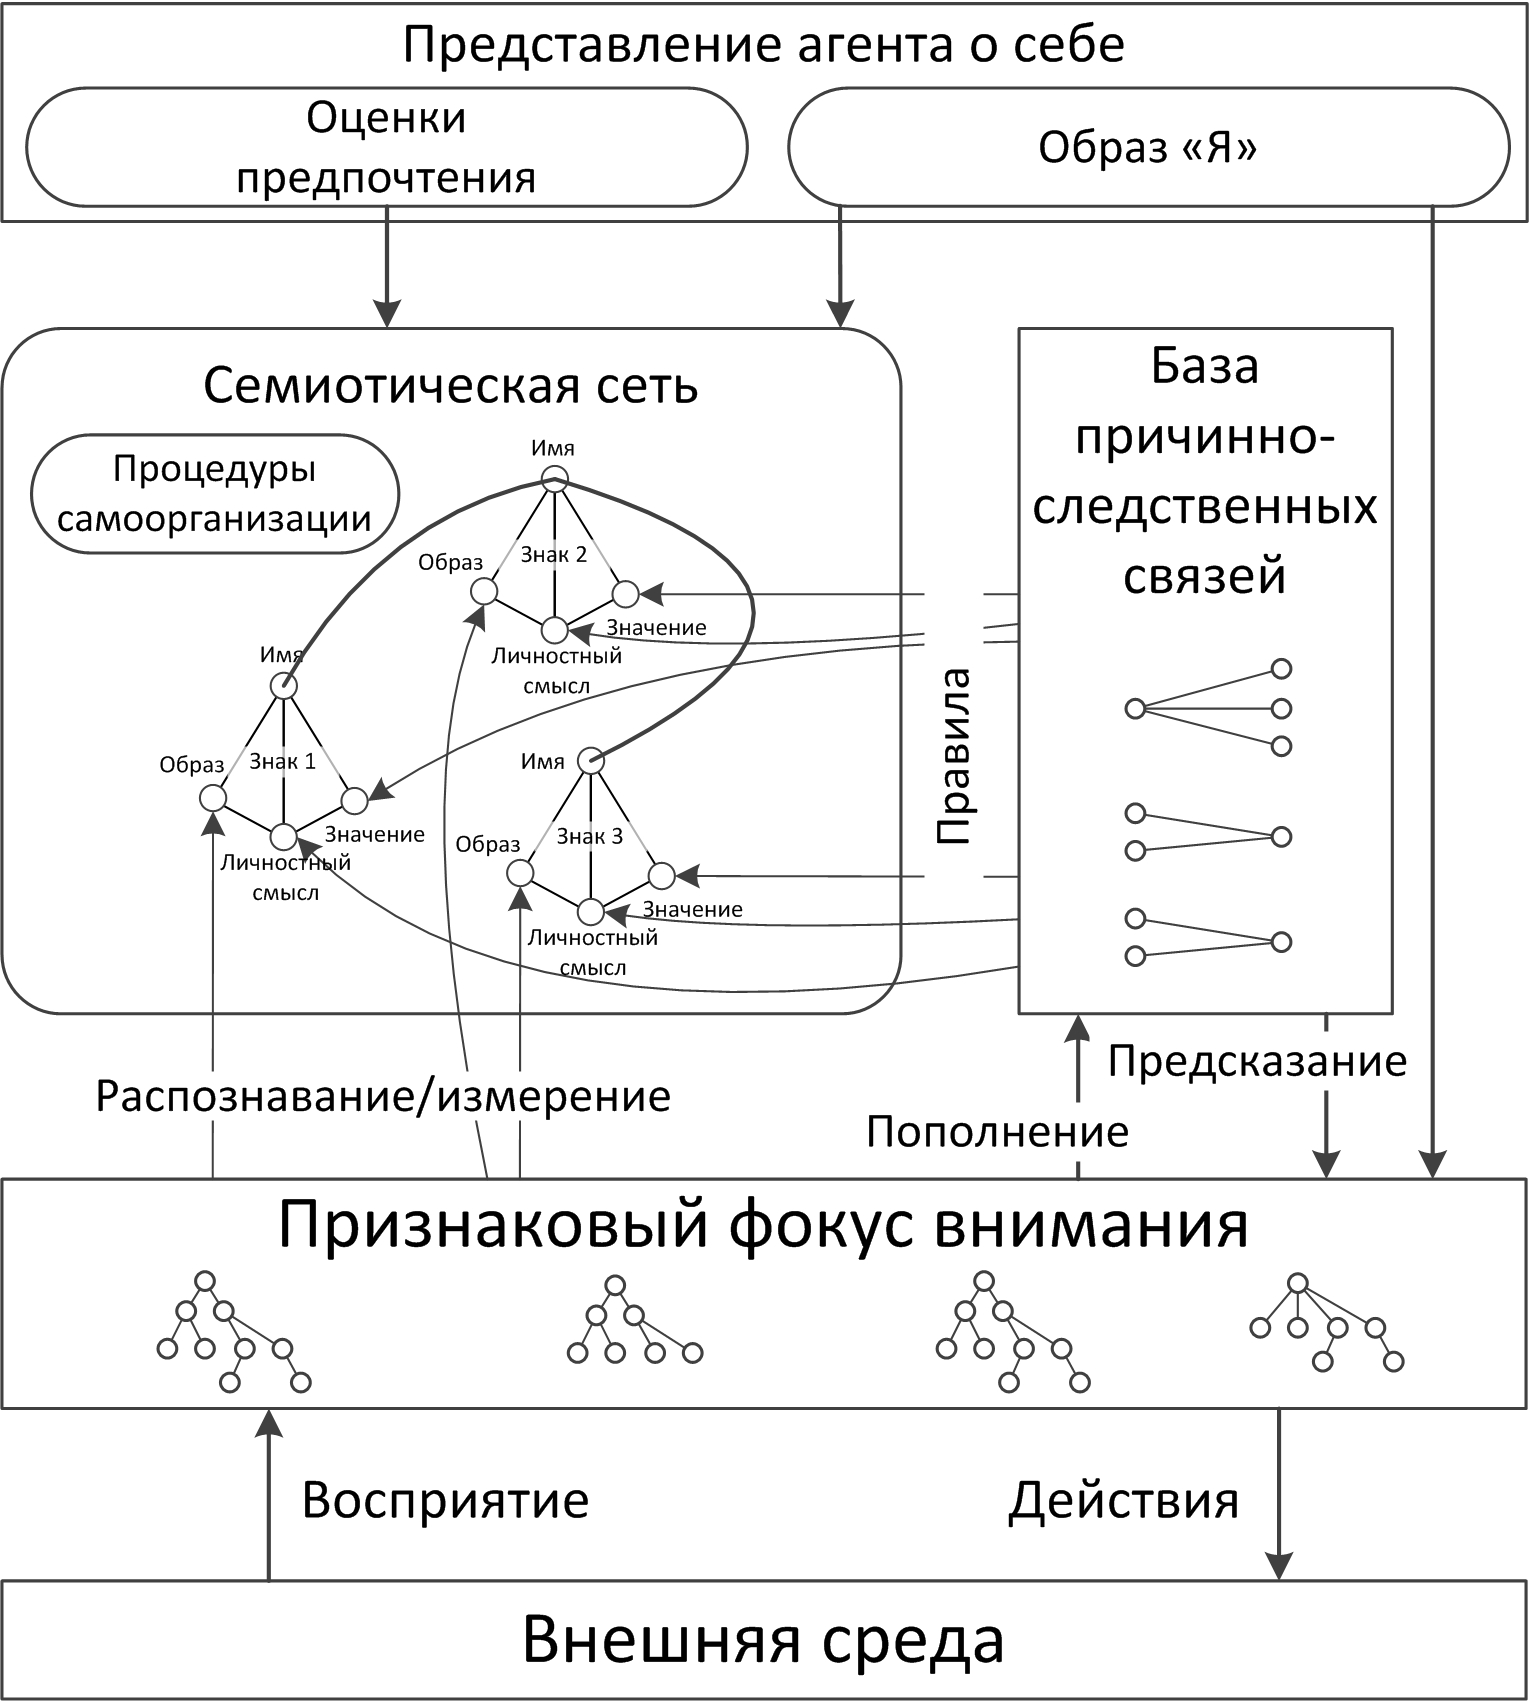
\includegraphics[width=0.7\linewidth]{iagent.jpg}
		\caption{Архитектура интеллектуального агента со знаковой картиной мира.}
		\label{fig:iagent}
	\end{figure}

	\section*{Заключение} В настоящей работе рассмотрены механизмы формирования компонент знака, согласующиеся с современными представлениями нейрофизиологов о строении коры головного мозга человека. Подробно рассмотрен модельный или семантический уровень описания картины мира субъекта деятельности, даны определения компонент знака на этом уровне. Исследован алгоритм связывания двух компонент знака: образа и значения, доказана его сходимость. Описаны особенности процессов планирования в картинах мира разных типов, построен алгоритм синтеза плана поведения в житейской картине мира. Приведена архитектура интеллектуального агента, который обладает знаковой картиной мира и способен к составлению плана поведения и распределению ролей в коалиции.
	
%	\noindent\colorbox{yellow}{
%		\parbox{\dimexpr\linewidth-2\fboxsep}{Про архитектуру агентов и распределение ролей.}
%	}
	
	\titleformat{\section}{\normalfont\centering\MakeUppercase}{\thesection.}{1pt}{}[]
	
	%	\nocite{*}
	\bibliography{../../biblio/umain}

\end{document}